
%%%%%%%%%%%%%%%%%%%%%%%%%%%  5  %%%%%%%%%%%%%%%%%%%%%%%%%%% 
\subsection{A high-speed network interface for distributed-memory systems: architecture and applications \cite{steenkiste1997high}} \label{ss:steenkiste1997high}
%%%%%%%%%%%%%%%%%%%%%%%%%%%  5  %%%%%%%%%%%%%%%%%%%%%%%%%%% 

\Accs{dmm} have not been successful in using the \acc{hippi} protocol.
Application on distributed system have very diverse I/O requirements.
% \Ac{hippi} support a data rate of 1.6 Gb/second. in traditional shard-memory supercomputers.
The problem lies in the high-speed I/O for \ac{dmm}, this is due to the systems working optimally in a distributed fashion while connected to an inherent sequential system.
An approach to network I/O on \ac{dmm} is to make the network interface responsible for network processing.
However, this is hard to do, because of potentially thousands of connected processor.
This approach could be improved by doing some of the communication overhead sensitive activities on the distributed-memory system.

\motive
There is a bottleneck in communication on \acs{dmm} which needs to be reduced.

\objective
An I/O architecture is created that supports high-speed I/O using a simple network interface to solve this problem.

\summary
\Ac{dmm}s communicate through a network interface that is connect both to the external network and the internal interconnect of the system (see: \cref{fig:rep4:conndistrmem}).

High speed I/O for \ac{dmm} is difficult because the system is designed to operate in a distributed fashion where serialization is avoided as much as possible.
It is hard to implement the following tasks on a \ac{dmm}: the communication protocol does not parallelize well, resources need to be scheduled, data that needs to be send/received is typically divided of the private memories of the  nodes.
These processing tasks roughly correspond to the OSI network model (see: \cref{fig:rep4:osi}).


\begin{figure}
	\centering
	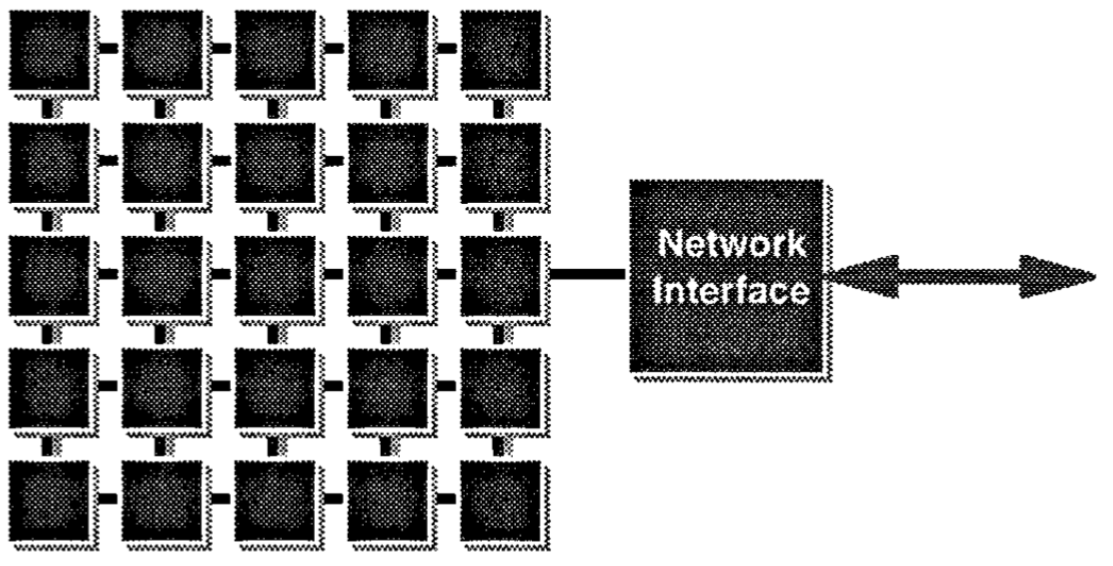
\includegraphics[width=0.95\linewidth]{Figures/Rep4DistrMemSys.png}
	\caption{Connecting a distributed-memory system to a network., Source: \cite{steenkiste1997high}.} 
    \label{fig:rep4:conndistrmem}
\end{figure}

\begin{figure}
	\centering
	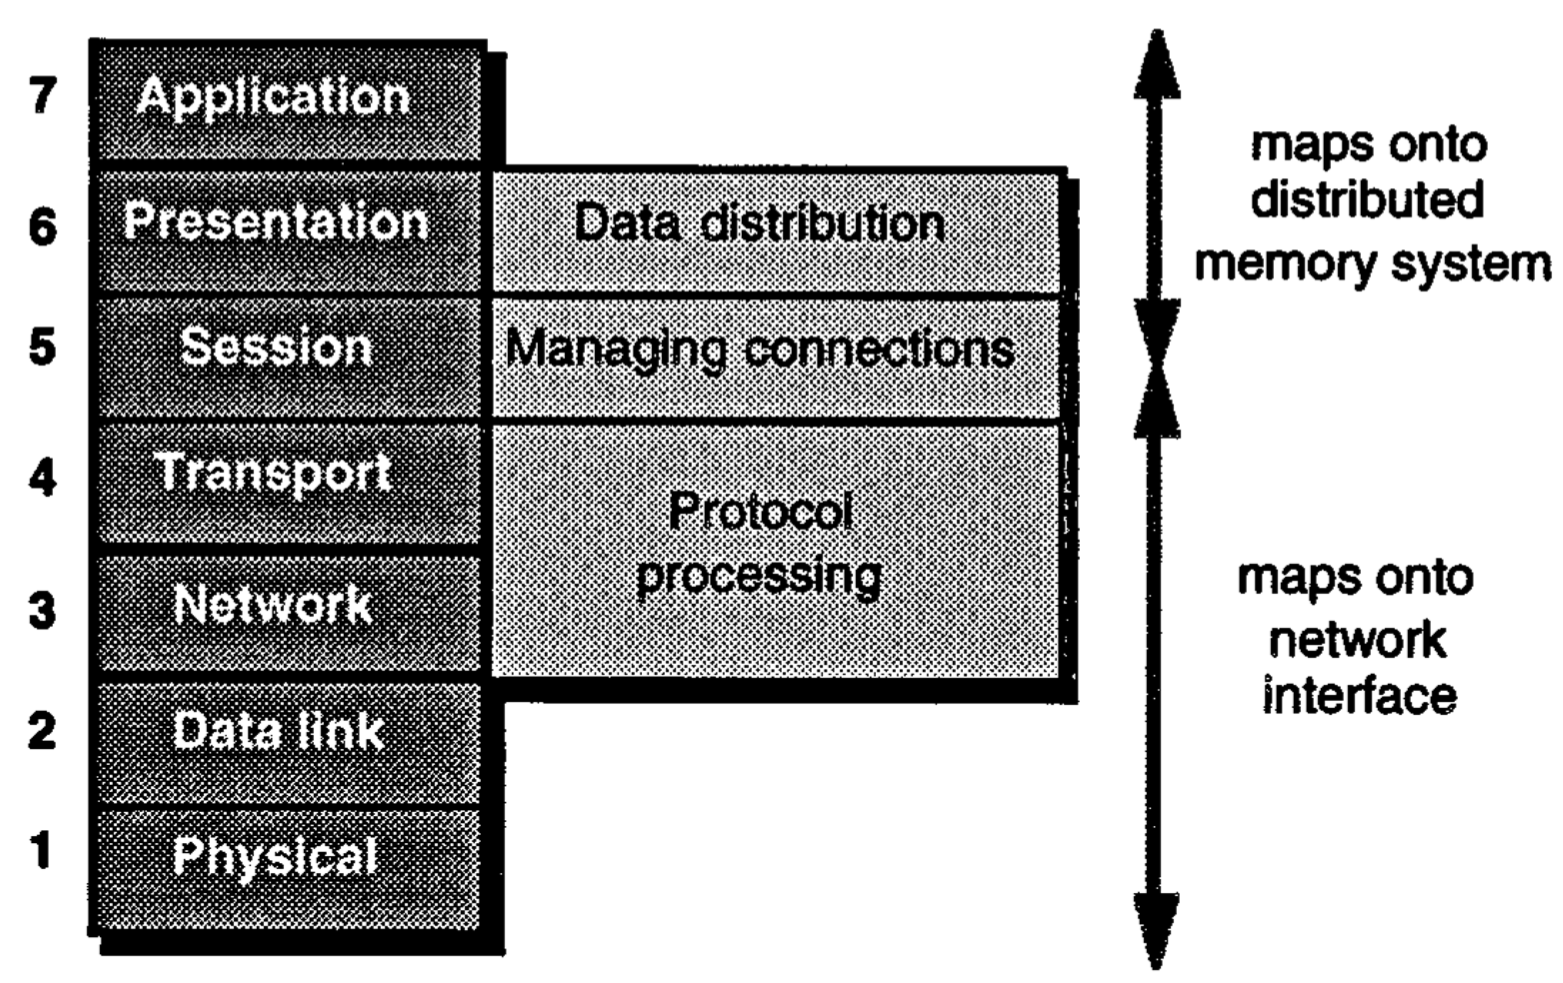
\includegraphics[width=0.95\linewidth]{Figures/Rep4OSI.png}
	\caption{Mapping of the protocol stack., Source: \cite{steenkiste1997high}.} 
    \label{fig:rep4:osi}
\end{figure}